\section{研究方法、技术路线、实验方案}
\subsection{研究方法}
\begin{frame}{\insertsection}{\insertsubsection}
	\begin{center}
		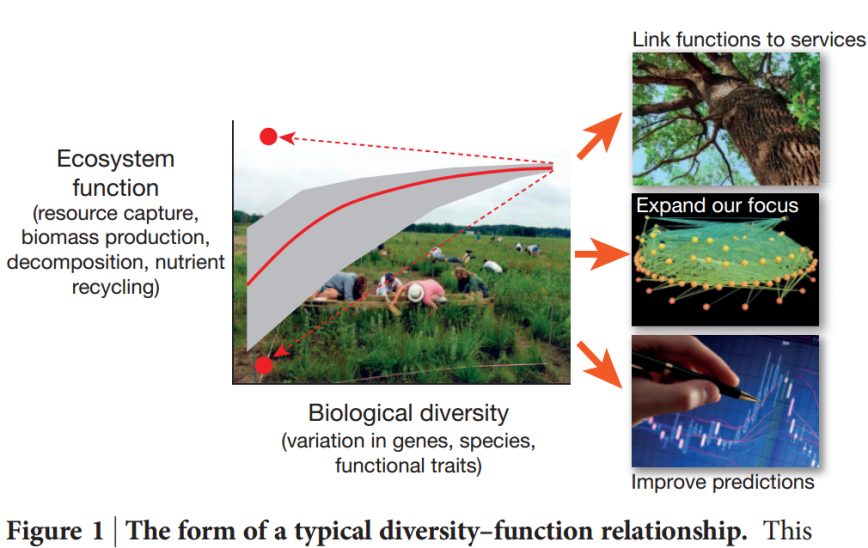
\includegraphics[width = 0.9\textwidth]{./pic/2.1.1.png}
	\end{center}
1)植物多样性梯度;
2)土壤微生物多样性梯度;\\
3)演替梯度;
4)环境因子梯度;\\
5)功能群移除;
\end{frame}
\begin{frame}{\insertsection}{\insertsubsection}
	\begin{center}
		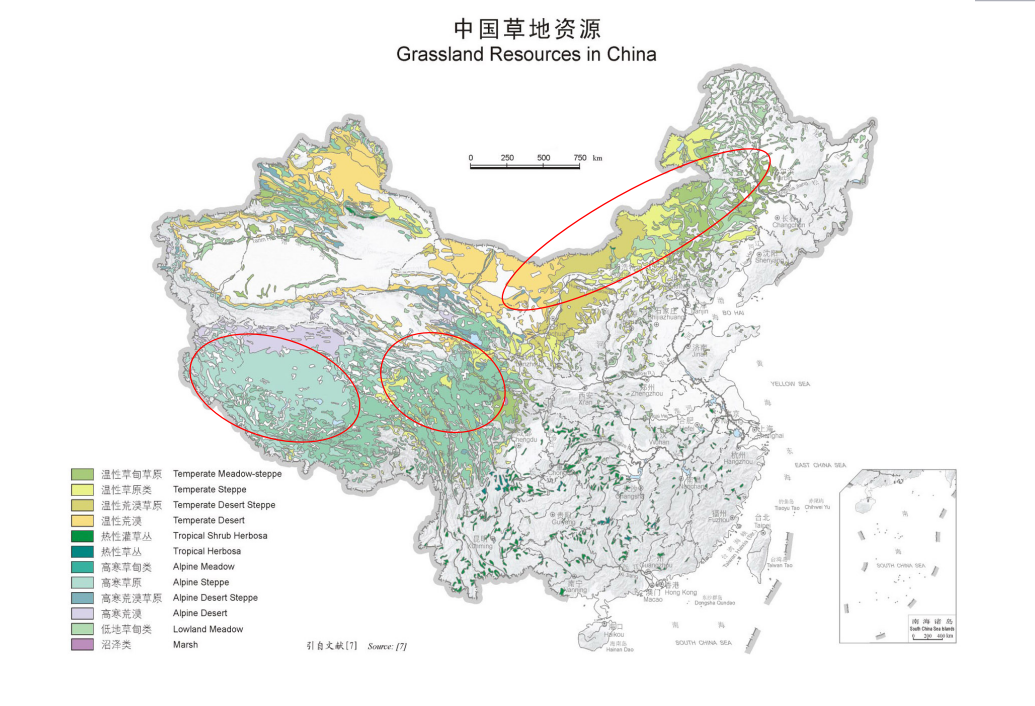
\includegraphics[width = 0.9\textwidth]{./pic/2.1.2.png}
	\end{center}
	研究地点:
	
	西藏、青海、内蒙古南北两条平行样带
\end{frame}
\begin{frame}{\insertsection}{\insertsubsection}
	土壤理化性质参数
	
	把样带采集的土壤过筛(1mm×1mm)除去根,置于背光条件下自然风干备用。
	
	1)TOC;2)TN;3)TP;4)MBC;5)MBN;6)NH4-N;7)NO3-N;8)有效P;9)pH
\end{frame}
\begin{frame}{\insertsection}{\insertsubsection}
	植物多样性参数
	
	α多样性:丰富度指数(Richness)、Shannon-Winer多样性指数(H')
	
	(1)
	
	式(1)中S为物种数,Pi为第i种个体所占总个体数的比例。
\end{frame}
\begin{frame}{\insertsection}{\insertsubsection}
	植物多样性参数
	
	β多样性:Bray-Curtis指数:
	
	(2)
	
	式(2)中,jI为样地A(jI a)和样地B(jI b)共有种物种重要值较小者之和;
	
	(3)
	
	式(3)中,aI、bI分别为样地A和B物种重要值。
\end{frame}
\begin{frame}{\insertsection}{\insertsubsection}
	室内试验
	
		\begin{center}
			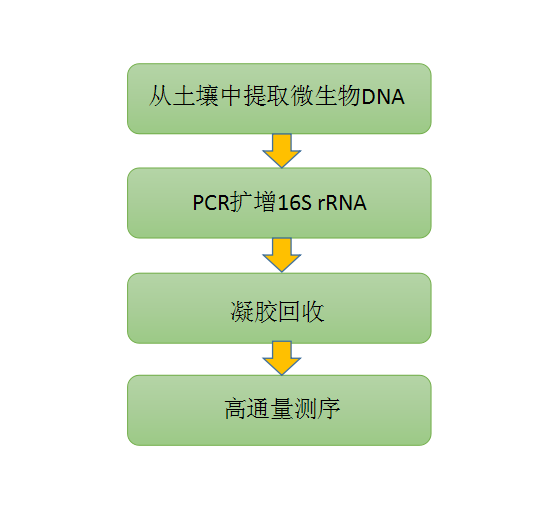
\includegraphics[width = 0.6\textwidth]{./pic/2.1.3.png}
		\end{center}
\end{frame}


\subsection{技术路线}
\begin{frame}{\insertsection}{\insertsubsection}
	\begin{center}
		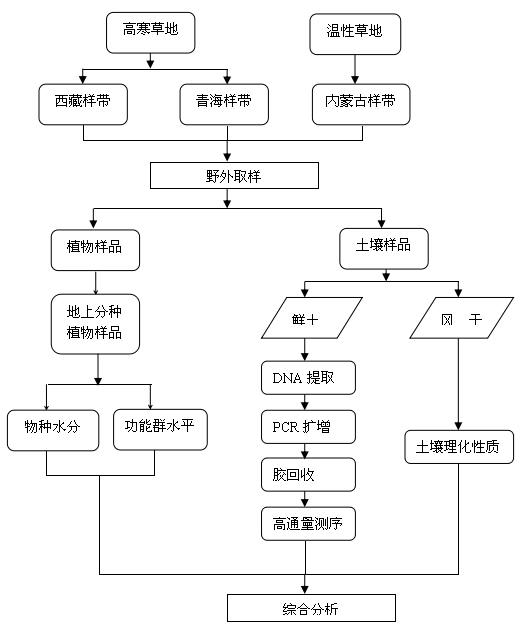
\includegraphics[width = 0.6\textwidth]{./pic/技术路线.jpg}
	\end{center}
\end{frame}
\subsection{实验方案}
\begin{frame}{\insertsection}{\insertsubsection}
	\begin{center}
		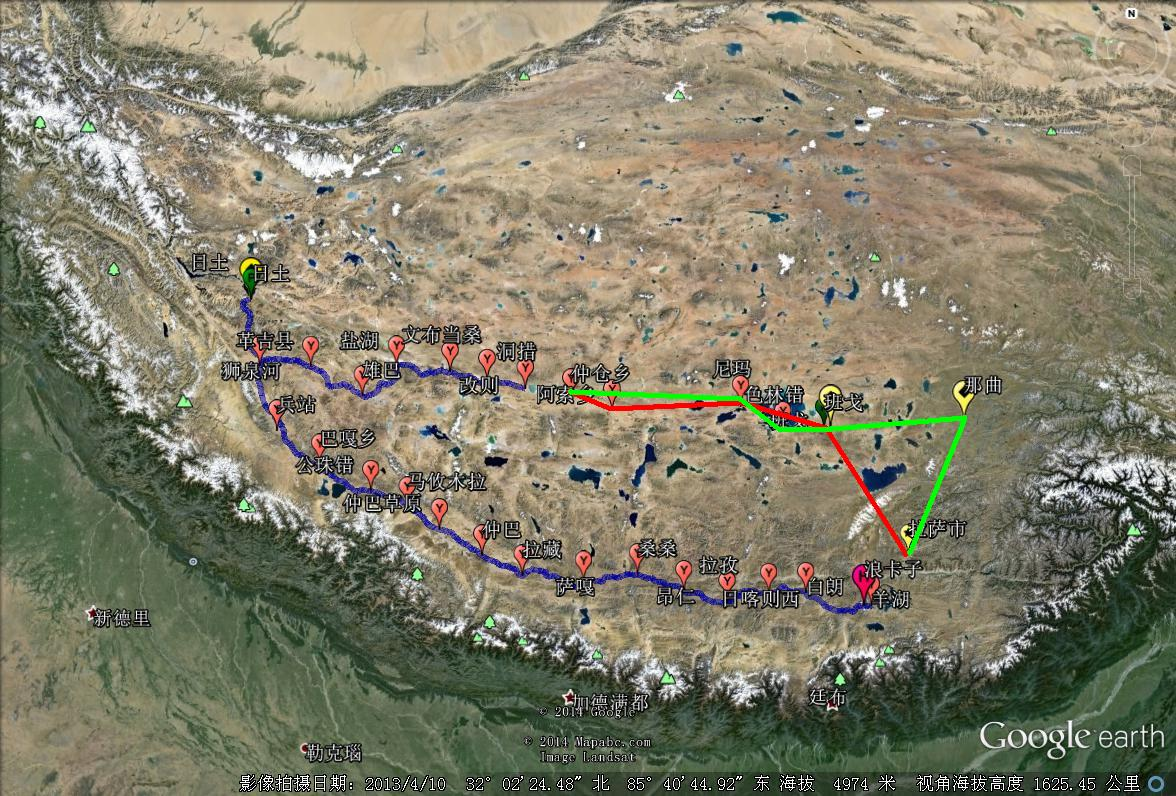
\includegraphics[width = 0.9\textwidth]{./pic/西藏瓦岗.jpg}
	\end{center}
	1)在西藏冈底斯山脉南北两侧,沿水分梯度各由东往西定点取样;
\end{frame}

\begin{frame}{\insertsection}{\insertsubsection}	
	\begin{columns}
		\column{0.5\textwidth}
		\begin{center}
			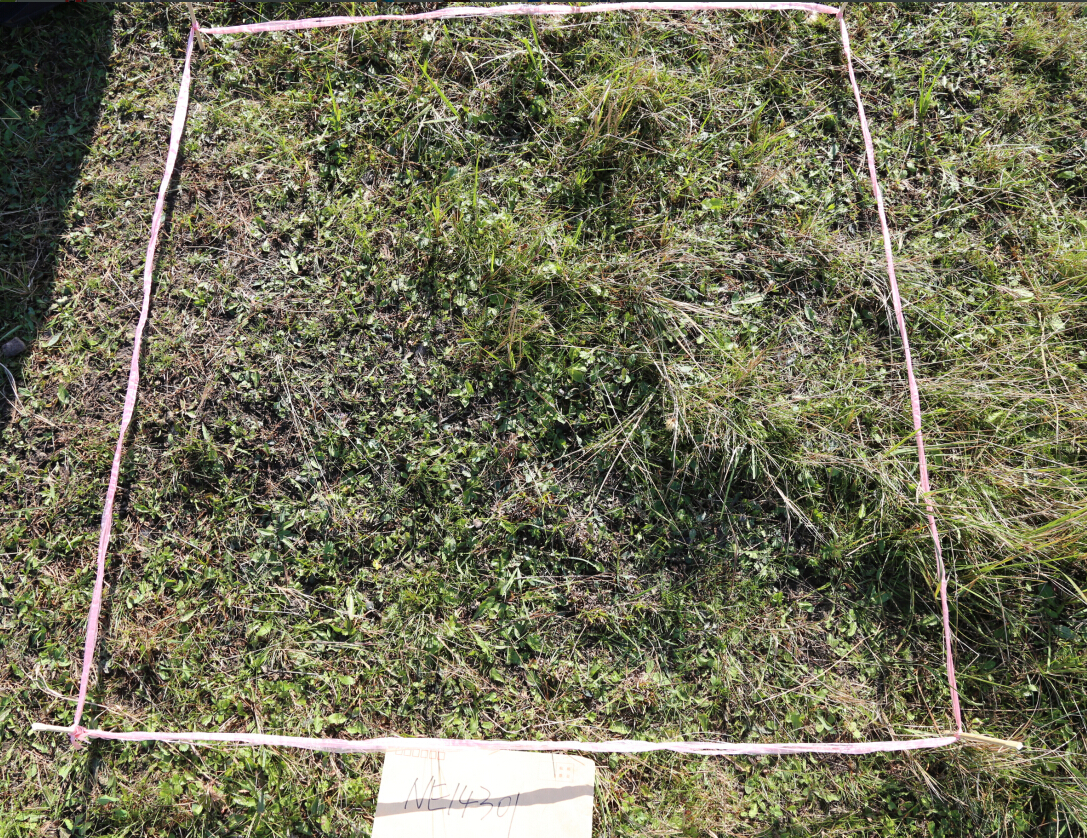
\includegraphics[width = 1.1\textwidth]{./pic/2.3.1.jpg}
		\end{center}		
		\column{0.5\textwidth}
		\begin{center}
			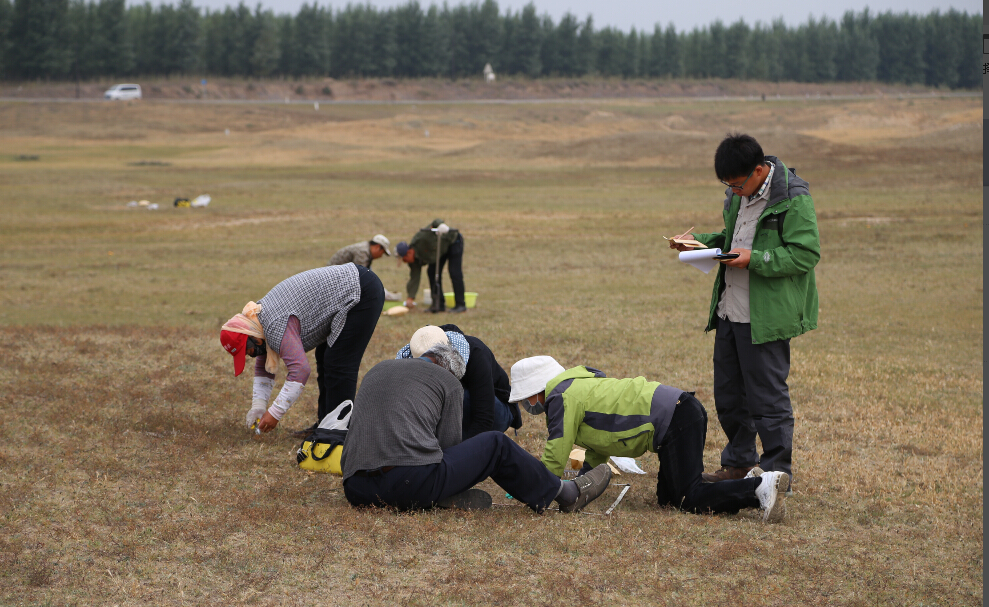
\includegraphics[width = 1.4\textwidth]{./pic/2.3.2.jpg}
		\end{center}
	\end{columns}
	\vskip 2em
	2)在每个取样点,随机选择5个1m×1m的样方,记录每个物种(随机选取5株)的高度,分种剪取地上植物生物量,称鲜重,实验室65℃烘72小时,称干重;	
\end{frame}
\begin{frame}{\insertsection}{\insertsubsection}	
	\begin{columns}
		\column{0.5\textwidth}
		\begin{center}
			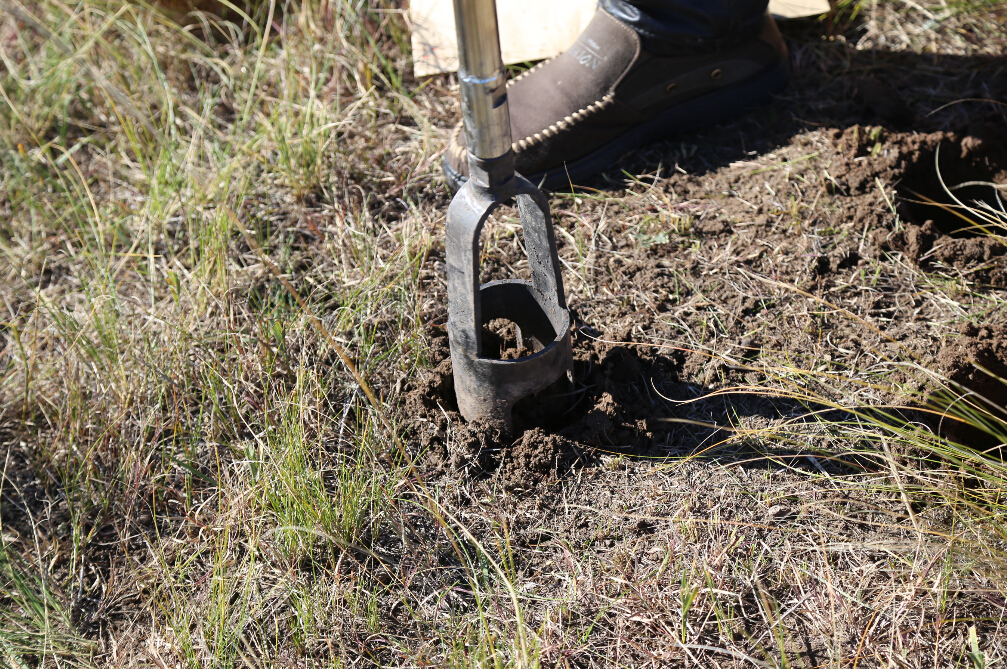
\includegraphics[width = 1.1\textwidth]{./pic/2.3.3.jpg}
		\end{center}		
		\column{0.5\textwidth}	
		\begin{center}
			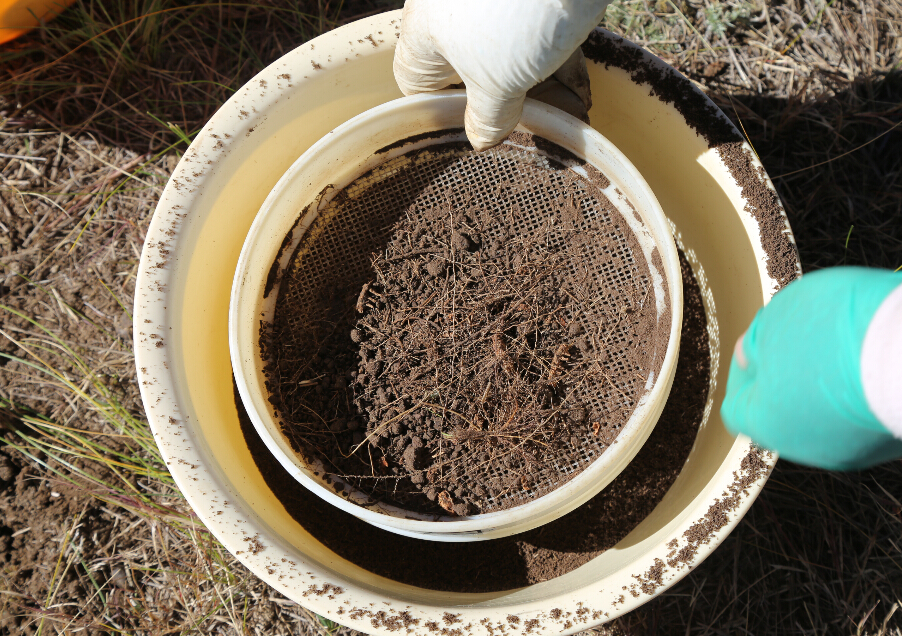
\includegraphics[width = 1.05\textwidth]{./pic/2.3.4.jpg}
		\end{center}
	\end{columns}
	\vskip 2em
	3)在每个取样点随即选择的5个1m×1m的样方剪除地上生物量后,用5cm根钻每层(0-10cm、10-20cm、20-30cm)取3钻土壤样品并均匀混合,一半土壤样品迅速放入野外冰箱并冷冻保存,用于提取微生物DNA;另外一半带回实验室风干,用于测量土壤的理化性质;	
\end{frame}

\begin{frame}{\insertsection}{\insertsubsection}
\begin{center}
	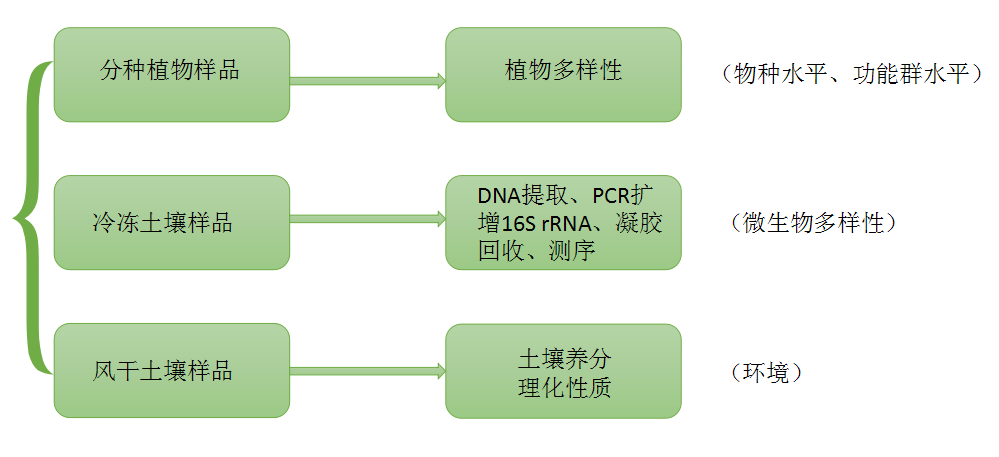
\includegraphics[width = 1.1\textwidth]{./pic/2.3.5.png}
\end{center}
\end{frame}


